\documentclass[tikz,border=10pt]{standalone}
\begin{document}
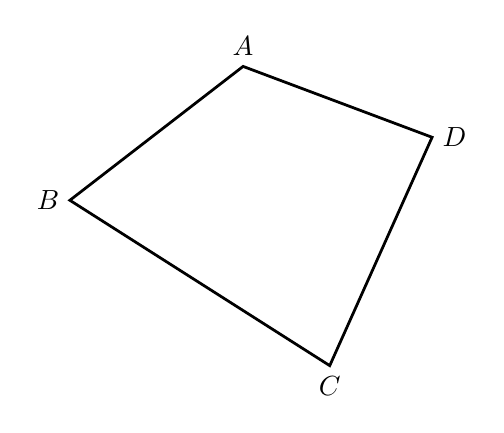
\begin{tikzpicture}[line width=1pt]
\coordinate (A) at (2.2,3.5);
\coordinate (B) at (0,1.8);
\coordinate (C) at (3.3,-0.3);
\coordinate (D) at (4.6,2.6);

\draw (A) -- (B) -- (C) -- (D) -- cycle;

\node[above] at (A) {$A$};
\node[left] at (B) {$B$};
\node[below] at (C) {$C$};
\node[right] at (D) {$D$};
\end{tikzpicture}
\end{document}
